\documentclass[12pt]{article}

\title{AMath Tea Time --- Puzzle #1}

\begin{document}

\maketitle

{\it Hello, everyone! I thought it would be nice to have a weekly mathematical
  and programming puzzles to accompany our tea time activities. I don't want to
  puzzle to discourage people from talking with each other; quite the opposite!
  The weekly puzzle is meant to be discussed!

  I'll post new puzzles every Tuesday and add hints on Thursday.

  --
  Chris S.}

\subsection*{Problem}

There are 2015 airports in the far away land of Dijkstrania. Every pair of
airports is connected by a nonstop flight in one or both directions. Show that
there is some airport from which it is possible to reach evey other airport in
at most two flights.

\begin{figure}[H]
  \centering
  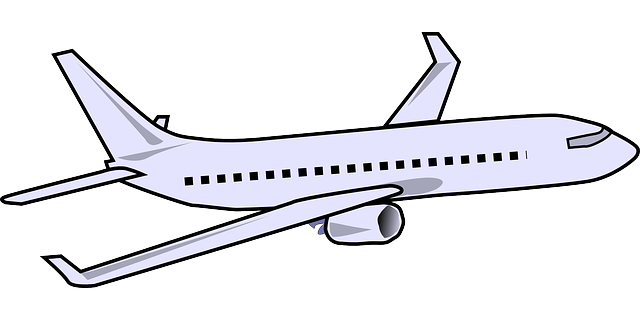
\includegraphics{airplane.png}
\end{figure}

\subsection*{Hints}

{\it (Hints will be written here on Thursday.)}

\vspace{6cm}

\subsection*{Suggestions?}

If you have any suggested mathematical or programming puzzles to share then send
them my way at {\tt cswiercz@gmail.com}!

\end{document}
